%\part{Aspectos Gerais}
\chapter[Referencial Teórico]{Referencial Teórico}
Visando facilitar o entendimento acerca dos principais temas desta pesquisa, este capítulo define os aspectos e elementos relacionados a sistema de
recomendação, perfil de testadores, testes exploratórios e governo digital.
%---------------- Governo Digital ---------------------%
\section{Governo Digital}

O advento da internet surgiu e reconfigurou o meio de comunicação para a população e, através do advento da evolução da tecnologia 
e expansão da internet surge a expressão \textit{Governo Digital}. Esta expressão se refere ao uso de tecnologias digitais como uma 
estratégia de modernização de um Governo, que adota a tecnologia da informação e comunicação (TIC) para prover 
serviços~\cite{fang2002government}. 

O termo \textit{e-Governo} surgiu no final da década de 1990 e cresceu consideravelmente com 
diversas definições como: governo mais eficiente, melhores serviços para o cidadão e um melhor processo 
democrático. Em sequência, nos últimos anos, o termo \textit{e-Governo} deu origem a várias conferências de cunho científico, aumentando seu 
conteúdo e posição no que se refere a outros campos de pesquisa e disciplinas~\cite{gronlund2005introducing}.

A OECD (Organisation for Economic Co-operation and Development) usa a expressão \textit {Governo Eletrônico} como o uso de 
Tecnologias de Informação e Comunicação pelo governo, que se refere a uma ferramenta que busca melhorar as atividades do governo, 
especialmente, através do uso da Internet. A expressão \textit{Governo Digital}, por outro lado, refere-se ao uso de tecnologias 
digitais que buscam adicionar valor público como parte complementar às estratégias de modernização de um governo.

A integração de novas tecnologias no cotidiano faz com que as expectativas dos cidadãos sobre suas relações com os governos mudem 
\cite{oecd}, visto que as opiniões e necessidades podem passar a ser consideradas de forma mais eficaz, trazendo a possibilidade 
de realizar processos mais facilmente. Esta consolidação das expectativas criadas sobre o governo exige que novas abordagens de governança pública possam trazer a digitização de serviços,
considerando-se que, atráves da desburocratização de alguns serviços e processos, os cidadãos e empresas podem estar integrados ao
meio digital.

Embora as medidas de modernização do setor público tenham começado a ser adotadas na década de 70, a dedicação, de fato, 
apareceu apenas em decorrência da crise fiscal dos anos 80, quando a intervenção estatal se popularizou como reforma da gestão 
pública que, aliada às TICs, disponibilizou serviços públicos eletrônicos à população no início da década de 2000~\cite{przeybilovicz2015desenvolvimento}.

No Brasil, em 2016, somente 54\% dos domicílios brasileiros possuiam acesso à internet, o que representa 6,7 milhões de residências
e um total de 107,9 milhões de usuários de Internet~\cite{CGI}. Neste mesmo ano, ocorreu o lançamento da \textit{Estratégia de Governança Digital da Administração Pública Federal} (EGD),
com o objetivo de definir estratégias, metas e indicadores da Política de Governança Digital. A partir da EGD, a prestação de serviços
públicos poderia ser simplificada e agilizada proporcionando uma melhoria no ambiente de negócios e eficiência da gestão pública.

Ainda em 2016, o Decreto número 8.638 foi publicado pela Casa Civil da Presidência da República (BRASIL2016c), instituindo a 
Política de Governança Digital, no âmbito dos órgãos e das entidades da administração pública federal direta, autárquica e 
fundacional. 

No Decreto número 8.638 (BRASIL2016c), existem dois artigos a serem destacados por seus princípios e obetivos, estes estão 
listados na tabela a seguir:

% Please add the following required packages to your document preamble:
% \usepackage{graphicx}
% \usepackage[table,xcdraw]{xcolor}
% If you use beamer only pass "xcolor=table" option, i.e. \documentclass[xcolor=table]{beamer}
    \begin{table}[h]
        \resizebox{\textwidth}{!}{%
        \begin{tabular}{cc}
        \hline
        {\color[HTML]{000000} \textbf{Artigo 1º do Decreto}} & {\color[HTML]{000000} \textbf{Artigo 3º do Decreto}} \\ \hline
        Benefícios para a sociedade & Necessidades da sociedade \\
        Participação da sociedade & Simplicidade e inovação \\
        Obtenção de informações pela sociedade & Serviços públicos em meio digital \\ \hline
        \end{tabular}%
        }
        \end{table}

Para estimular a transformação dos serviços públicos em serviços digitais, de modo que estes ocorram por meio eletrônico, o governo
brasileiro publicou decretos relevantes entre 2014 e 2016, como citado ao longo desta seção. Os decretos definira, a Política de Governança
Digital e a Plataforma de Cidadania Digital, no no âmbito da Administração Pública Federal (APF), ambos de responsabilidade do 
Ministério do Planejamento, Desenvolvimento e Gestão (MP) anos (BRASIL 2016a, b). 

A Plataforma de Cidadania Digital configura um conjunto de metodologias e soluções que buscam ampliar, simplificar o acesso dos
cidadãos aos serviços digitais e, também, para apoiar os órgãos públicos na aceleração da transformação digital de serviços. 

Simultaneamente às ações da Plataforma de Cidadania Digital, o Departamento lançou um canal para oferecer informações no
formato de um  portal de serviços do Governo Federal. A iniciativa surgiu para permitir o arquivamento de solicitações eletrônicas 
e monitorar os serviços públicos pelos usuários. Juntamente com o portal, foi lançado um programa de automação de serviços 
públicos, para a tentativa de orientar e apoiar órgãos públicos a identificar, priorizar, digitalizar e implementar serviços 
com mais qualidade e transparência para os cidadãos.

Um dos objetivos do governo brasileiro com a transformação digital é ampliar os serviços públicos nos canais digitais. 
Atualmente, o governo oferece aproximadamente 1.700 serviços, mas apenas 41\% são totalmente digitais.

Tendo em vista os decretos publicados, o Departamento INOVA do antigo MP, se responsabilizou pela construção
de um programa de Governo Digital, denominado \textit{Kit de Transformação}. O objetivo é, de modo geral, transformar os serviços públicos através de um kit,
ao invés da adoção de uma metodologia, por exemplo, objetivando facilitar a adoção e orientação aos diversos órgãos da APF.

O \textit{Kit de Transformação} é composto por seis estágios de aplicações independentes, como demonstra a figura X.

\begin{figure}[h]
    \centering
    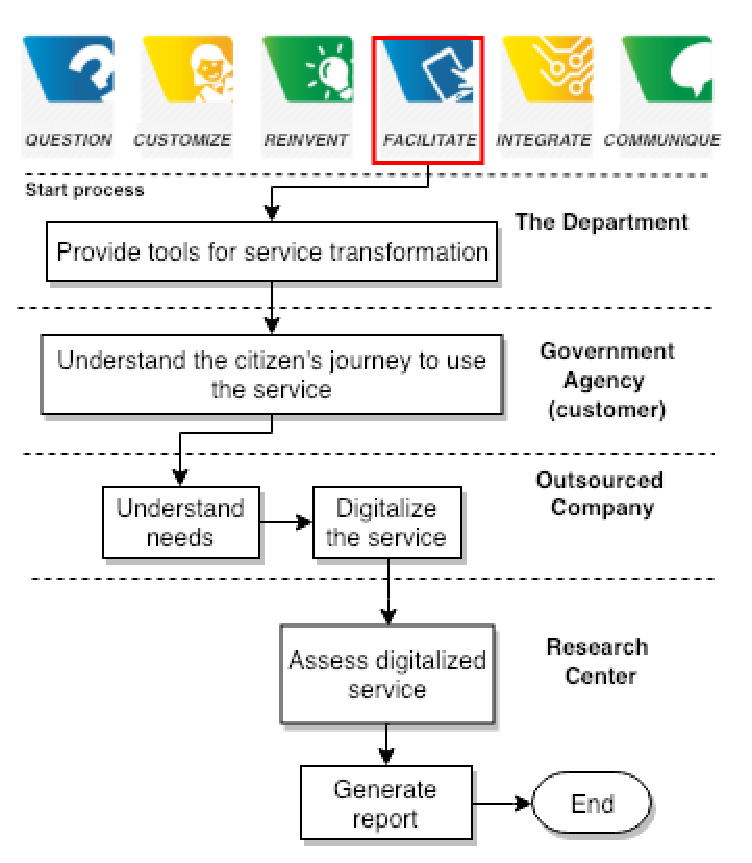
\includegraphics{figuras/kitTransformacao.eps}
    \caption[Referencial Teórico]{Kit de Transformação e seus estágios de aplicação.}
    \label{img:kitTransformacao}
\end{figure}


%---------------- Testes Exploratórios-----------------%

\section{Testes exploratórios}

Os testes exploratórios foram mostrados na indústria de software com seus primeiros materiais produzidos 
aparecendo em blogs da internet~\cite{kaner2000testing} e, em 2009, apareceu em livros texto. 

O termo também aparece em SWEBOK~\cite{bourque2014guide}, onde é definido simultaneamente como aprendizagem, o projeto de teste 
e a execução do teste, ou seja, os testes são definidos antecipadamente em um plano de teste estabelecido, mas 
são dinamicamente projetados, executados e modificados.

Dentro dessa abordagem de teste existem etapas de design de teste e execução, onde os testadores estão constantemente aprendendo e 
adaptando o design e a execução de resultados, o que promove a abertura de crenças de que o teste exploratório tenha cobertura de 
teste limitada em comparação com outros métodos de teste~\cite{schaefer2014model}.

Contudo, a automação de testes exploratórios pode resolver buscar a resolução da problemática da limitação, visto que testes 
automatizados podem reduzir a quantidade de tempo que os testadores podem gastar construindo casos de teste e executando-os, 
economizando, assim, tempo e dinheiro~\cite{dustin2009implementing}. 

%---------------- Sistema de Recomendação--------------%

\section{Sistema de Recomendação}
